
\msection{\Wasm}

Starting with the Web 2.0 paradigm, JavaScript has long been the language for client-side scripting in modern web browsers. 
However, its complexity, security vulnerabilities, and performance limitations have led to the exploration of various alternatives for client-side scripting over the years \cite{javaapplet,activex,silverlight}. 
Remarkably, these alternatives largely failed to gain traction, primarily due to security concerns and a lack of consensus among browser vendors.

% asm.js and the demonstration of bad language patterns
In 2014, Alon Zakai and colleagues proposed Emscripten \cite{emscripten}. 
Emscripten used a strict subset of JavaScript, asm.js, to allow low-level code such as C to be compiled to JavaScript. 
This approach came with the benefits of having all the ahead-of-time optimizations from LLVM, gaining in performance on browser clients \cite{asmjs}.
Asm.js was faster than JavaScript because it limited the language features to those that can be optimized in the LLVM pipeline. 
Besides, it removed the majority of the dynamic characteristics of the language.
Since asm.js was a subset of JavaScript it was compatible with all engines at that moment. 
Asm.js demonstrated that client-code could be improved with the right language design and standardization.

%The work of Van Es \etal \cite{EsAsm.js} proposed to shrink JavaScript to asm.js in a source-to-source strategy, closing the cycle and demystifying the fact that asm.js was mainly a compilation target for C/C++ code. 
Following the asm.js initiative, the W3C publicly announced the \Wasm\ (Wasm) language in 2017. \wasm\ is a binary instruction format for a stack-based virtual machine and was officially consolidated by the work of Haas \etal \cite{Haas_2017} in 2017. 
The announcement of \wasm\ marked the first step into the standardization of bytecode in the web environment. 
Wasm is designed to be fast, portable, self-contained and secure, and it promises to outperform JavaScript execution \cite{Haas_2017}. 
Since 2017, the adoption of \wasm\ keeps growing. For example; Adobe, announced a full online version of Photoshop\footnote{\url{https://twitter.com/Adobe/status/1453034805004685313?s=20&t=Zf1N7-WmzecA0K4V8R69lw}} written in WebAssembly;  game companies moved their development from JavaScript to Wasm like is the case of a full Minecraft version\footnote{\url{https://satoshinm.github.io/NetCraft/}}; and the case of Blazor\footnote{\url{https://dotnet.microsoft.com/en-us/apps/aspnet/web-apps/blazor}}, a .Net virtual machine implemented in Wasm, able to execute C\# code in the browser.


Moreover, WebAssembly has been evolving outside web browsers since its first announcement.
Some works demonstrated that using WebAssembly as an intermediate layer is better in terms of startup and memory usage than containerization and virtualization \cite{pMendkiServerless, 1244493Jacobsson}. 
Consequently, in 2019, the Bytecode Alliance \cite{bytecodealliance} proposed WebAssembly System Interface (WASI) \cite{WASI}. 
WASI pionered the execution of \wasm\ with a POSIX system interface protocol, making possible to execute Wasm directly in the operating system. 
Therefore, it standardizes the adoption of \wasm\ in heterogeneous platforms \cite{bryant2020webassembly}, making it suitable for edge-cloud computing platforms \cite{9640153, wen2020wasmachine}.

\msubsection{Binary format}
\label{background:wasm:binary}

A \Wasm binary usually consists of a single module that serves as the foundational unit for deployment, loading, and compilation. 
A \Wasm program requires a host environment for execution. 
This host is tasked with loading the \Wasm binary and allocating the necessary resources for its successful operation. 
The interaction between the engine and the \Wasm program is fundamentally dictated by the structure of the binary itself.
In essence, a \Wasm binary serves as a contract between the \Wasm program and the host engine. 
It comprises a mix of definitions and declarations that establish the rules of engagement. 
In this context, a declaration refers to a newly specified element, such as the bodies of functions inside the binary, while a definition refers to an element originating from the host, such as imported functions.

A \wasm binary is organized into sections, each with a distinct semantic role and specific placement within the module. 
This structured organization facilitates further machine code compilation. 
Table \ref{background:wasm:sections} provides a summary of these sections, detailing their ID, name, and purpose.
As illustrated in Figure \ref{background:wasm:fig:section}, a \Wasm section is a byte sequence that begins with a 1-byte section ID, followed by an 8-byte section size, and concludes with the section content, which matches the previously indicated size.


\begin{table}
    \centering
    \begin{tabular}{r l | p{8cm}}
    ID & Section Name & Description \\
    \midrule
    0 & Custom & Comprises two parts: the section name and arbitrary content. Primarily used for storing metadata, such as the compiler used to generate the binary. \\
    1 & Type & Contains the function signatures for functions declared or defined within the binary. \\
    2 & Import & Lists elements imported from the host, including functions, memories, globals, and tables. \\
    3 & Function & Details functions defined within the binary. Essentially maps Type section entries to Code section entries. \\
    4 & Table & Groups functions with identical signatures to control indirect calls. \\
    5 & Memory & Specifies the number and initial size of unmanaged linear memories. \\
    6 & Global & Defines global variables as managed memory for use and sharing between functions in the \Wasm binary. \\
    7 & Export & Declares elements like functions, globals, memories, and tables for host engine access. The entry point of the \Wasm binary is typically declared here. \\
    8 & Start & Designates a function to be called upon binary readiness, initializing the \Wasm program state before executing any exported functions. \\
    9 & Element & Contains elements to initialize the binary tables. \\
    10 & Code & Contains the body of functions defined in the Function section. Each entry consists of local variables used and a list of instructions. \\
    11 & Data & Holds data for initializing unmanaged linear memory. Each entry specifies the offset and data to be placed in memory. \\
    12 & Data Count & Primarily used for validating the Data Section. If the segment count in the Data Section mismatches the Data Count, the binary is considered malformed. \\
    \end{tabular}
    \caption{Overview of binary sections in \Wasm binaries, following the \Wasm 1.0 specification.}
    \label{background:wasm:sections}
\end{table}
    
    
    \begin{figure}
    \centering
    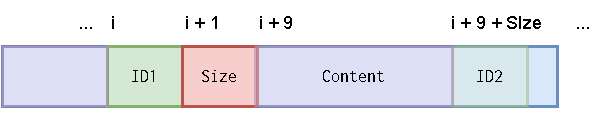
\includegraphics[width=0.5\linewidth]{figures/section.pdf}
    \caption{Memory byte representation of a \Wasm binary section, starting with a 1-byte section ID, followed by an 8-byte section size, and finally the section content.}
    \label{background:wasm:fig:section}
    \end{figure}
    


Some sections, like the Start and Custom sections, are optional, enhancing the binary's flexibility. 
The Custom section, for instance, can store metadata such as the compiler used. 
The modular format allows for efficient parsing; a compiler can skip irrelevant sections, speeding up the compilation process. 
Additionally, only a few sections have order constraints, offering further flexibility. Custom sections can even be repeated multiple times within the binary.

% Should we discuss the function body here?


\msubsection{\Wasm's Runtime structure}
\label{background:wasm:execution}

\todo{Reorder this text according with the wrules}

The \Wasm runtime structure is described in the WebAssembly specification by enunciating 10 key components: the Store, Stack, Locals, Module Instances, Function Instances, Table Instances, Memory Instances, Global Instances, Export Instances, and Import Instances. 
These components are particularly significant in maintaining the state of a WebAssembly program during its execution. 
In the following text, we provide a brief description of each runtime component.

\wrule{Store}: The WebAssembly store represents the global state and is a collection of instances of functions, tables, memories, and globals. Each of these instances is uniquely identified by an address, which is usually represented as an i32 integer.


\wrule{Module Instances}: A module instance is a runtime representation of a loaded and initialized WebAssembly module. 
It contains the runtime representation of all the definitions within a module, including functions, tables, memories, and globals, as well as the module's exports and imports.


\wrule{Table instances}: A table instance is a vector of function elements. 
WebAssembly tables are used to support indirect function calls.
For example, it allows modeling dynamic calls of functions (through pointers) from languages such as C/C++, for which the Wasm's compiler is in charge of populating the static table of functions.


\wrule{Export Instances}: Export instances represent the functions, tables, elements, globals or memories that are exported by a module. 

\wrule{Import Instances}: Import instances represent the functions, tables, elements, globals or memories that are imported into a module from the host. 

\wrule{The Stack} holds typed values and control frames, with control frames handling block instructions, loops, and function calls.
Values inside the stack can be of the only static types allowed in Wasm 1.0, \texttt{i32} for 32 bits signed integer, \texttt{i64} for 64 bits signed integer, \texttt{f32} for 32 bits float and \texttt{f64} for 64 bits float.
Therefore, abstract types, such as classes, objects, and arrays, are not natively supported. 
Instead, during compilation, such types are transformed into primitive types and stored in the linear memory.

\wrule{Memory Instances} represent the unmanaged linear memory of a WebAssembly program, consisting of a contiguous array of bytes.
Memory instances are accessed with \texttt{i32} pointers (integer of 32 bits). 
Memory instances are usually bound in browser engines to 4Gb of size, and it is only shareable between the process that instantiates the \Wasm module and the binary itself.

\wrule{Global Instances}: A global instance is a global variable with a value and a mutability flag, indicating whether the global can be modified or is immutable.
Global variables are part of the managed data, i.e., their allocation and memory placement are managed by the host engine.
Global variables are only accessible by their declaration index, and it is not possible to dynamically address them. 


\wrule{Locals}: Locals are mutable variables that are local to a specific function invocation. As globals, locals are part of the managed data.

\begin{note}\label{managed_unmanaged}
    Along with this dissertation, as the work of Lehmann \etal \cite{usenixWasm2020}, we refer to managed and unmanaged data to differentiate between the data that is managed by the host engine and the data that is managed by the \Wasm program respectively.
\end{note}

\wrule{Function Instances}: A function instance is a closure, which is the pairing of a function's code with a module instance. This pairing is required because the function's code might refer to other definitions within the module instance, such as globals, tables, or memories.
A function instance groups locals and a function body.
Locals are typed variables that are local to a specific function invocation.
The function body is a sequence of instructions that are executed when the function is called.
Each instruction either reads from the stack, writes to the stack, or modifies the control flow of the function.

\msubsection{Control flow}

In \Wasm, functions are organized into blocks, with the function's starting point serving as the root block. 
Unlike traditional assembly code, control flow structures in Wasm jump between block boundaries rather than arbitrary positions within the code. 
Each block might specify the required stack state before execution and the resulting stack state after its instructions have run. 
This stack state is used to validate the binary during compilation and to ensure that the stack is in a valid state before executing the block's instructions.
Blocks in Wasm are explicit, indicating, with instructions, where they start and end.

By design, each block operates autonomously and cannot reference or execute code from outer blocks. 
Control flow within a function is managed through three types of break instructions: unconditional break, conditional break, and table break. 
Importantly, each break instruction is limited to jumping to one of its enclosing blocks.

Loops in Wasm are specialized blocks that can be restarted using a break instruction. Unlike standard blocks, where breaks jump to the end of the block, breaks within a loop block jump to the block's beginning, effectively restarting the loop. 
To illustrate this, \autoref{background:wasm:block} provides an example comparing a standard block and a loop block in a Wasm function.


\begin{minipage}{0.95\linewidth}
   
   \begin{minipage}{0.45\linewidth}
      \lstset{
      language=WAT,
      style=WATStyle,
      breaklines=true, 
      %stepnumber=0,
      escapeinside={(*@}{@*)},
      numbers=none,
      postbreak=\mbox{\space},
      label=BlockExample}

   \begin{lstlisting}    
block
   block
      br 1 (*@\tikzmarkMap{2}{}{8.5}{2}{2cm}@*) ; Jump instructions are annotated with the depth of the block they jump to; 
   end (*@\tikzmarkMap{7}{}{8.5}{0}{2cm}@*)
end (*@\tikzmarkMap{1}{}{8}{3}{2cm}@*)
... (*@\tikzmarkMap{9}{}{8.5}{2}{2cm}@*)
   \end{lstlisting}
   \end{minipage}\hspace{1mm}
   \begin{minipage}{0.44\linewidth}
   \lstset{
      language=WAT,
      style=WATStyle,
      breaklines=true, 
      %stepnumber=0,
      escapeinside={(*@}{@*)},
      numbers=none,
      postbreak=\mbox{\space},
      label=LoopExample}

   \begin{lstlisting}    
loop (*@\tikzmarkMap{6}{}{8.5}{2}{2cm}@*)
   ...
   br 0 (*@\tikzmarkMap{5}{}{8.5}{2}{2cm}@*) ;first-order break;
   ... 
end (*@\tikzmarkMap{3}{}{8.5}{2}{2cm}@*) ; end instructions break the block and jump to next instruction; 
... (*@\tikzmarkMap{4}{}{8.5}{-2}{2cm}@*)
   \end{lstlisting}
   \end{minipage}
   \begin{tikzpicture}[remember picture,overlay]

      %\path (2.west) edge[<-, black] (1.west);
      %\path (3.west) edge[<-,  black] (4.west);
   
      \path (1.west) edge[<-, bend right, black] (2.west);
      %\path (1.west) edge[<-, bend right, gray] (7.west);
      %\path (9.west) edge[<-, bend right, gray] (1.west);
   
      \path (4.west) edge[<-, bend right, gray] (3.west);
      \path (6.west) edge[<-, bend left, black] (5.west);
      %\path (9.east) edge[<-, bend right, black] (4.east);
      %\path (7.east) edge[<-, bend right, black] (8.east);
   
      \end{tikzpicture}
      \centering
      \hrule
      \vspace{2mm}
      \captionof{lstlisting}{Example of breaking a block and a loop in \Wasm.}
      \label{background:wasm:block}
\end{minipage}
% Example


Each break instruction includes the depth of the enclosing block as an operand. 
This depth is used to identify the target block for the break instruction. 
For example, in the left-most part of the previously discussed listing, a break instruction with a depth of 1 would jump past two enclosing blocks.


For the purposes of this dissertation, we introduce a specific term to describe a particular kind of break within loops:

\begin{definition}\label{first_order_jump}
Break instructions within loops that effectively jump to the loop's beginning are termed \emph{first-order breaks}.
\end{definition}


\msubsection{From Source Code to Wasm }

\todo{Replace by Rust example}
\todo{Annotate the Wasm code with the sections offset and length}
\todo{Instantiate each one of the previously mentioned concepts}

% Example and intro to the stack
In \autoref{CExample1} and \autoref{WASMExample} we illustrate a C program and the Wasm program that results from its compilation. 
The C function contains: heap allocation, external function declaration and the definition of a function with a loop, conditional branching, function calls and memory accesses. 
The code in \autoref{WASMExample} shows the textual format for the generated Wasm. 
The module in this case first defines the signature of the functions (\lineref{tpe1}, \lineref{tpe2}  and  \lineref{tpe3})  that help in the validation of the binary defining its parameter and result types. The information exchange between the host and the Wasm  binary might be in two ways, exporting and importing functions, memory and globals to and from the host engine (\lineref{import1}, \lineref{export1} and \lineref{export2}). The definition of the function (\lineref{func1}) and its body follows the last import declaration at \lineref{import1}. 


% Example
\begin{code}
    \begin{minipage}[b]{0.45\linewidth}
        \lstset{language=C,caption={Example C function.},
        label=CExample1,
        breaklines=true, 
        basicstyle=\small\ttfamily,
        captionpos=b,
        frame=b,
        numbers=none,
        postbreak=\mbox{\textcolor{red}{$\hookrightarrow$}\space},
        escapeinside={(*@}{@*)}
        }
\input{sota/code/code.c}
\end{minipage}\hspace{10mm}
\begin{minipage}[b]{0.46\linewidth}
\lstset{
    language=WAT,
    caption={\wasm\ code  for \autoref{CExample1}.},
    style=WATStyle,
    breaklines=true, 
    %stepnumber=0,
    captionpos=b,
    frame=b,
    escapeinside={(*@}{@*)},
    numbers=none,
    postbreak=\mbox{\textcolor{red}{$\hookrightarrow$}\space},
    label=WASMExample}
%
\input{sota/code/code.fix.wat}
%\end{lstlisting}
\end{minipage}


%\begin{tikzpicture}[remember picture,overlay]

%\path (2.west) edge[<-, black] (1.west);
%\path (3.west) edge[<-,  black] (4.west);

%\path (6.east) edge[<-, bend right, black] (3.east);
%\path (9.east) edge[<-, bend right, black] (4.east);
%\path (7.east) edge[<-, bend right, black] (8.east);


%\end{tikzpicture}
\end{code}


% Functions
The function body is composed of local-variable declarations and typed instructions that are evaluated using a virtual stack (Line 7 to Line 32 in \autoref{WASMExample}). Each instruction reads its operands from the stack and pushes back the result. The result of a function call is the top value of the stack at the end of the execution. In the case of \autoref{WASMExample}, the result value of the main function is the calculation of the last instruction, \texttt{i32.add} at \lineref{result}. 
As the listing shows, instructions are annotated with a numeric type.


\msubsection{WebAssembly's Ecosystem}
\label{background:wasm:ecosystems}

\todo{Go deep into the details of the tools that are comoing from parts of the jury}

\Wasm programs are pre-compiled from an array of source languages and are designed for execution in host environments such as web browsers.
Though the execution of a \Wasm program might be considered its final lifecycle stage, the \Wasm ecosystem is far from simplistic.
It comprises multiple stakeholders and a rich array of tools that cater to various needs.
In the subsequent text, we describe the \Wasm ecosystem by separating it into skateholders categories.

\wrule{Producers}, such as compilers, transform source code into \Wasm binaries. 
For example, LLVM has offered \Wasm as a backend option since its 7.1.0 release\footnote{\url{https://github.com/llvm/llvm-project/releases/tag/llvmorg-7.1.0}}, supporting a diverse set of frontend languages like C/C++, Rust, Go, and AssemblyScript\footnote{A subset of the TypeScript language}.
In parallel developments, the KMM framework\cite{kmm} has incorporated \Wasm as a compilation target, and the Javy approach\cite{Javy} focuses on encapsulating JavaScript code within isolated \Wasm binaries. 
This is achieved by porting both the engine and the source code into a secure \Wasm environment. 
Blazor also enables the compilation of C# code into \Wasm binaries for browser execution\footnote{\url{https://dotnet.microsoft.com/apps/aspnet/web-apps/blazor}}.
Regardless of the source language or framework, the resulting \Wasm binary functions similar to a traditional shared library, replete with code instructions, symbols, and exported functions.
%From a security standpoint, \Wasm programs are designed without a standard library and are prohibited from direct interactions with the operating system. Instead, the host environment offers a predefined set of functions that can be imported into the \Wasm program. 
%It falls upon the producers to specify which functions from the host environment will be imported by the \Wasm application.

\wrule{Consumers} encompass tools that undertake the tasks of validating, analyzing, transpiling to machine code, and executing \Wasm binaries, e.g. browser clients. 
In the text that follows, we dissect them into specific categories and their respective domains of application.

\todo{Locate WasmA} \cite{WasmA}

\wrule{Static and dynamic analysis, optimization and validation:} The toolkit for analysing \Wasm binaries is rich and varied. 
Tools such as Wassail\cite{wassail}, Wasmati\cite{wasmati}, and Wasp\cite{Wasp} utilize a range of methodologies, including information flow control, code property graphs, and concolic execution, to identify vulnerabilities. 
Dynamic analysis counterparts like TaintAssembly\cite{taintassembly}, Wasabi\cite{wasabi}, and Fuzzm\cite{fuzzm} serve analogous functions.
\todo{Add veriwasm}
\todo{Binanryen}

\wrule{Browsers} Engines like V8\cite{v8}, SpiderMonkey\cite{spidermonkey}, and Chakra\cite{chakra} are at the forefront of executing \Wasm binaries. 
These engines leverage Just-In-Time (JIT) compilers to convert \Wasm into machine code. 
This translation is typically a straightforward one-to-one mapping, given that \Wasm is already an optimized format closely aligned with machine code. 
For example, V8 employs quick, rudimentary optimizations such as constant folding and dead code removal\footnote{This analysis was corroborated through discussions with the V8 development team and through empirical studies in one of our contributions\cite{CROW}}. 

\wrule{Standalone engines} \Wasm's applicability has transcended browser environments, largely due to the WebAssembly System Interface (WASI)\cite{WASI}. 
WASI aims to standardize the interaction between host environments and \Wasm modules, thereby facilitating portability of both bytecode and binaries across diverse platforms. 
It outlines a POSIX-like Application Binary Interface (ABI), which includes functionalities for filesystem access, network sockets, clocks, and random number generation, among others. 
Standalone engines such as WASM3\cite{wasm3}, wasmtime\cite{wasmtime}, WAVM\cite{WAVM} and Sledge \cite{Sledge} have emerged to support \Wasm.
Similarly, Singh and colleagues \cite{WARDuino2019} proposed a virtual machine for Wasm in Arduino based devices.


\todo{Disect them into, JIT compilers and interpreters, ending with SWAM.}
\todo{Add the verifiable standalone engine here}

\wrule{Specialized Malware Detection} In niche areas like cryptomalware detection, tools like MineSweeper\cite{Minesweeper}, MinerRay\cite{MinerRay}, and MINOS\cite{MINOS} utilize static analysis techniques. 
Conversely, dynamic analysis is the forte of tools like SEISMIC\cite{SEISMIC}, RAPID\cite{RAPID}, and OUTGuard\cite{outguard}.

\wrule{Smart Contract Analysis} In the field of smart contracts, static analysis tools like EvalHunter\cite{evalhunter}, WANA\cite{wana}, and EOSAFE\cite{eosafe} are employed to unearth vulnerabilities in \Wasm-based contracts. Dynamic analysis tools in this sphere include EOSFuzzer\cite{eosfuzzer} and wasai\cite{wasai}.


\wrule{Obfuscation, and binary rewriting tools} \todo{WASMixer, Wobfuscator}

While many existing tools purport to offer self-correctness evaluations and exhaustive test suites, the \Wasm ecosystem is still in its early stages. 
To emphasize this, a 2021 study by Hilbig et al.\cite{Hilbig2021AnES} found a mere 8,000 unique \Wasm binaries globally. 
This pales in comparison to mature ecosystems like JavaScript and Python, which offer 1.5 million and 1.7 million packages on npm\footnote{\url{https://www.npmjs.com/}} and PyPI\footnote{\url{https://pypi.org/}}, respectively.
This limited pool of \Wasm binaries presents a unique challenge for machine learning-based analysis tools, which require large datasets for effective training. 
This issue is explicitly addressed in one of the contributions of this dissertation\cite{EVASION}.
Additionally, the scarcity of \Wasm programs exacerbates the problem of software monoculture, increasing the likelihood of consuming a compromised \Wasm program\cite{YourCitationHere}.
Besides, the current size of the \Wasm ecosystem offers a small testing environment for evaluating the capabilities of consumer tools.
This dissertation aims to address these issues by introducing a comprehensive suite of tools. 
These tools are crafted to not only bolster the security of \Wasm programs through Software Diversification but also to intensify the testing rigor for both producers and consumers in the ecosystem.


To the best of our knowledge, the most complete survey about Wasm  tooling is presented in the Awesome Wasm  (\url{https://github.com/mbasso/awesome-wasm}) repo. It is a cumulative GitHub repo which includes references to articles, papers, books, demos, compilers and engines related to \wasm. 


\msubsection{WebAssembly's Security}

\todo{Check the attack primitives defined by Lehmann.}

As we described, \wasm\ is deterministic and well-typed, follows a structured control flow and explicitly separates its linear memory model, global variables and the execution stack. This design is robust \cite{WebAssemblySecurity} and makes it easy for compilers and engines to sandbox the execution of Wasm  binaries. Following the specification of Wasm  for typing, memory, virtual stack and function calling,
host environments should provide protection against data corruption, code injection, and return-oriented programming (ROP).

However, implementations in both browsers and standalone runtimes~\cite{Narayan2021Swivel} are vulnerable.
Genkin \etal demonstrated that Wasm  could be used to exfiltrate data using cache timing-side channels \cite{Genkin2018DrivebyKC}.
Moreover, binaries itself can be vulnerable. The work of Lehmann \etal ~\cite{usenixWasm2020} proved that C/C++ source code vulnerabilities can propagate to Wasm  such as overwriting constant data or manipulating the heap by overflowing the stack. Even though these vulnerabilities need a specific standard library implementation to be exploited, they make a call for better defenses for \wasm. 
Recently, Stiévenart and colleagues demonstrate that C/C++ source code vulnerabilities can be ported to Wasm \cite{DeRoover2022}.
% Current proposals
Several proposals for extending \wasm\ in the current roadmap could address some existing vulnerabilities. For example, having multiple memories\footnote{\url{https://github.com/WebAssembly/multi-memory/blob/main/proposals/multi-memory/Overview.md}} could incorporate more than one memory, stack and global spaces, shrinking the attack surface. However, the implementation, adoption and settlement of the proposals are far from being a reality in all browser vendors\footnote{\url{https://webassembly.org/roadmap/}}. 
% In fact, according to the work of Hilbig \etal \cite{Hilbig2021AnES}, the artificial variants created with one of our works contribute to the half of executable and available \wasm\ binaries in the wild.
